\documentclass{article}

\author{Pedro Henrique Limeira da Cruz}
\title{ET520 - Conversão de Energia}

\usepackage[margin=0.8in]{geometry}
\usepackage{indentfirst}
\usepackage{fancyhdr}
\usepackage{tcolorbox} 
\usepackage{graphicx}
\usepackage{amsmath}
\usepackage{amssymb}
\usepackage{enumitem}
\usepackage{tabularx} % in the preamble


% Create a Todo list
\newlist{todolist}{itemize}{2}
\setlist[todolist]{label=$\square$}

\newcolumntype{Y}{>{\centering\arraybackslash}X}

% Create a new command to be used in the align environment in multiple line equations do only the last equation is numbered  
\newcommand{\n}{\nonumber \\ }
\makeatletter
\let\inserttitle\@title
\makeatother
% Set the style of the page 
\pagestyle{fancy}
\fancyhf{}
\rhead{Pedro Henrique L. da Cruz}
\lhead{\inserttitle}
\rfoot{Page \thepage}

\usepackage{hyperref}
\hypersetup{
    colorlinks=true,
    linkcolor=black,
    filecolor=magenta,
    urlcolor=cyan,
}

% Begin the Document 
\begin{document}

\maketitle
\thispagestyle{empty}

% Add the image inside a figure in as the first page
% \begin{figure}[h]
%     \begin{center}
%         
\includegraphics[scale = 0.15]{/Users/pedrocruz/Documents/UNICAMP/ES101/ES101 - Robotic Arm/img/unicamp.png}
%     \end{center}
% \end{figure}

% Change to the Next page 
\newpage
\tableofcontents
\newpage

\section{Introdução}
De modo geral, existem quatro princípios de como os campos magnéticos são utilizados em máquinas elétricas, sendo eles:

\begin{itemize}
    \item \textbf{Produção de Campo - Simples}: Um fio conduzindo uma corrente elétrica produz um campo magnético sem sua vizinhança.
    \item \textbf{Ação Transformador}: Um campo magnético variável no tempo induzirá uma tensão em uma bobina se este campo passar através de dela.
    \item \textbf{Ação Motor}: Um fio conduzindo corrente elétrica, na presença de um campo magnético, tem uma força induzida sobre ele.
    \item \textbf{Ação Gerador}: Um fio movendo-se na presença de um campo magnético tem uma tensão induzida nele.
\end{itemize}

Para que possamos entender melhor sobre cada um dos princípios acima, precisamos primeiro sermos capazes de representar as diferentes topologias que estão envolvidas e simplificar as contas, através da criação de modelos. 

Como temos muita familiarização com os modelos criados para circuitos, iremos criar um paralelo entre circuitos elétricos e o que chamaremos de \emph{circuitos magnéticos}.


\section{Circuitos Magnéticos}
\subsection{Produção de Campo Magnético}
\subsubsection{Relação $i-H$}

Antes de vermos a representação e simbologias utilizadas para os modelos de circuitos magnéticos, precisamos primeiro entender como eles são gerados.


\begin{wrapfigure}{r}{0.3\textwidth}
    \centering
    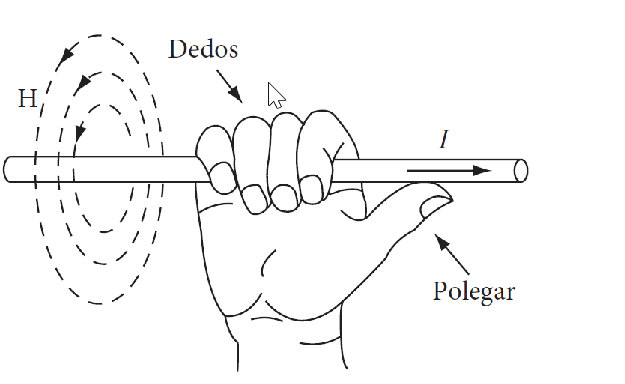
\includegraphics[width=0.3\textwidth]{imgs/2023-08-15 10_18_18-1_CIRCUITOS_MAG.pdf - ET520 - Princípios de Conversão de Energia - Visual Studio.png}
    \caption{Regra da Mão Direita}
    \label{img:regra_da_mao_direita}
\end{wrapfigure}

Como dito na listagem dos princípios magnéticos (no começo do capítulo), um \textbf{campo é gerado sempre que uma corrente passa em um condutor}, onde a direção de tal campo pode ser determinado pela direção da corrente (utilizando da regra da mão direita, como mostrado na imagem \ref{img:regra_da_mao_direita}).

Partindo do axioma acima, conseguimos modelar matematicamente a relação entre campo e corrente, mis especificamente a relação entre a \textbf{Intensidade de Campo Magnético $H$} e corrente:
\begin{align}
    \oint \vec H \cdot \vec{dl} = i_{net}
\end{align}

Onde:
\begin{itemize}
    \item $\vec H$: Representa o vetor Intensidade de Campo.
    \item $\vec{dl}$: Representa o vetor comprimento do elemento infinitesimal de fio sob análise.
    \item $i_{net}$: Representa a corrente resultante, utilizada se há mais de um frio conduzindo corrente. 
\end{itemize}

Desenvolvendo essa integral de linha, para um caso simplificado onde a linha é representada por um circulo de raio $r$, temos:

\begin{wrapfigure}{r}{0.3\textwidth}
    \centering
    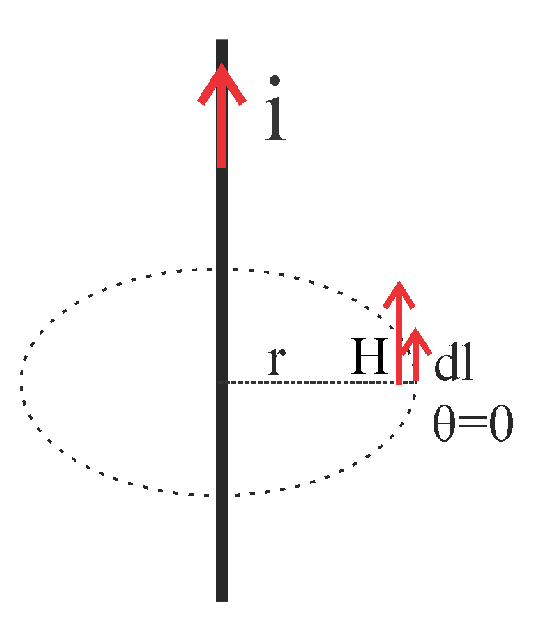
\includegraphics[width=0.3\textwidth]{imgs/2023-08-15 11_04_26-1_CIRCUITOS_MAG.pdf - ET520 - Princípios de Conversão de Energia - Visual Studio.png}
    \caption{Calculo - Intensidade $H$}
\end{wrapfigure}

\begin{align}
    &\oint \vec H \cdot \vec{dl} = i \n
    &\oint  H dl \cos \theta = i , \ \  \vec H \parallel \vec{dl} \therefore \theta = 0 \n
    &\oint  H dl = i \n 
    &H \oint  dl = i \n 
    &H 2 \pi r = i \n 
    &H = \frac{i}{2 \pi r }
\end{align}

Para o caso específico de espiras, podemos ainda relacionar a intensidade $H$ com a corrente e a quantidade de voltas dada:
\begin{align}
    \oint \vec H \cdot \vec{dl} = Ni \n
    H l = Ni
    \label{eq:intensidade_espiras}
\end{align}

Onde o $l$ representa o perímetro "planificado" da área na qual foi enrolada a espira, isso é, no caso de um toroid de raio $r$, no qual foram feitas $N$ voltas de fio, o $l$ é dado por $l=2\pi r$.

É importante ter em mente que a intensidade $H$ representa o \textbf{esforço} que a corrente precisa fazer para estabelecer um campo magnético.

\subsubsection{Relação $H-B$}
A intensidade $H$ do campo produz uma densidade de fluxo $B$ em todos os pontos que existe, dada por: 
\begin{align}
    B = \mu H
\end{align}

Onde $\mu$ representa a \textbf{Permeabilidade Magnética}, referente ao material no qual a intensidade está gerando a densidade magnética. Normalmente, entretanto, essa permeabilidade tem valores muito extremos (tanto para mais, como no caso de materiais ferro-magnéticos, quanto para menos, como no caso do vácuo $\approx$ ar), por isso nós usualmente utilizamos:

\begin{align}
    B = \mu_{relative} \mu{Vac} H
\end{align}

Onde $\mu{r} = \mu{relative}$ é a permeabilidade magnética do material relativo (i.e divide) a permeabilidade do vácuo $\mu_{0} = \mu_{vac} = 4\pi 10^{-7}$. Como consequência, para a análise de densidade no vácuo, ar, isloantes ou condutores elétricos (como cobre ou alumínio) o $\mu \approx \mu_0 \therefore \mu_r = 1$.

Além disso, é interessante analisar a relação entre permeabilidade ($\mu$), intensidade ($H$) e densidade ($B$):

\begin{align*}
    B = \mu H \Rightarrow \begin{cases}
        B = const & \downarrow \mu \therefore \uparrow H \\ 
        H = const & \downarrow \mu \therefore \downarrow B
    \end{cases}
\end{align*}

\subsubsection{Fluxo Magnético}

De uma forma geral, somos capazes de calcular o \textbf{fluxo magnético} $\Phi$, passando por um core magnético no cenário onde não há leakage \footnote{leakage é o fenômeno onde parte do fluxo de campo passar por fora do core e é perdido} pela equação:
\begin{align}
    \Phi = B A_C
\end{align}

Onde $A_C$ representa a área, constante, do core ferro-magnético.


\subsubsection{Circuito Magnético Equivalente}
Agora que temos as equações básicas para calcularmos os principais elementos magnéticos, iremos fazer o paralelo com os circuitos elétricos, começando pela  \textbf{Força Magneto Motriz} $\mathcal{F}$, que faz o paralelo com a tensão em circuitos convencionais.
\begin{align}
    \mathcal{F} = Hl = \underbrace{Ni}_{Espiras}
\end{align}

Onde, para o caso de espiras, o $N$ representa a quantidade de voltas, como mostrado na equação \ref{eq:intensidade_espiras}.

A partir disso, podemos fazer, então, o paralelo da lei de Ohm para circuitos magnéticos, sendo ele:
\begin{align}
    \Phi &= B A \n 
         &= (\mu H) A \n 
         &= \frac{\mu N i}{l} A \Leftarrow Hl = Ni \therefore H = Ni/l \n
         &= \frac{\mu N i}{l} A \frac{1/(\mu A)}{1/(\mu A)} \n
         &= \frac{N i}{l/(\mu A)} \n
         &= \frac{\mathcal{F}}{\mathcal{R}}
\end{align}

Onde chamamos o $\mathcal{R}$ de \textbf{Relutância}.

\begin{wrapfigure}{r}{0.3\textwidth}
    \centering
    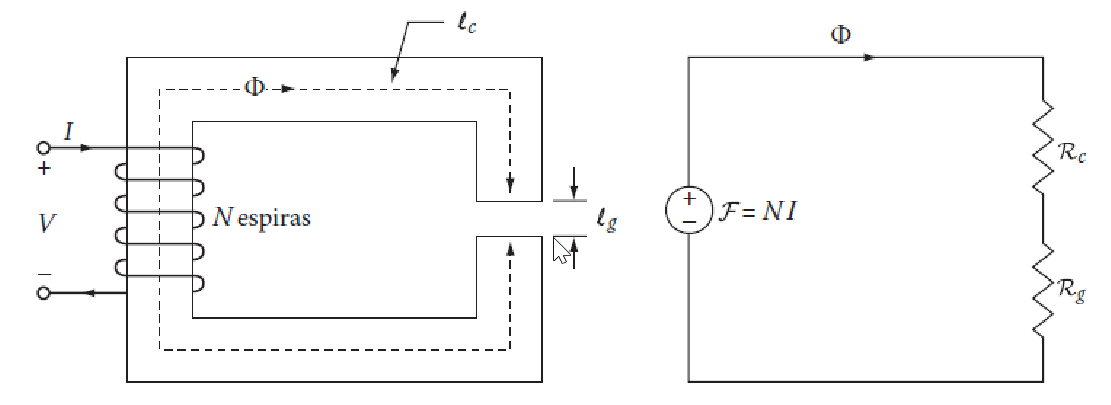
\includegraphics[width=0.3\textwidth]{imgs/circuito_equivalente.png}
    \caption{Circuito Equivalente}
    \label{img:circuito_equivalente}
\end{wrapfigure}

A partir desses conceitos, nós somos capazes de resolver problemas relativamente complexos, ao representarmos ele como um circuito magnético, com uma força magneto motriz (referenciando uma tenção), relutâncias (referenciando resistências, sendo que cada materias/estágio do circuito magnético possui um) e um fluxo magnético (que tem como contrapartida a corrente elétrica), como podemos ver pela image \ref{img:circuito_equivalente}.

Para resolvermos 

\end{document}